\documentclass[11pt, oneside]{article} 
\usepackage{geometry}
\geometry{letterpaper} 
\usepackage{graphicx}
	
\usepackage{amssymb}
\usepackage{amsmath}
\usepackage{parskip}
\usepackage{color}
\usepackage{hyperref}

\graphicspath{{/Users/telliott/Dropbox/Github-Math/quickgeo/figures/}{/Users/telliott/Dropbox/Github-Math/figures/}}
% \begin{center} \includegraphics [scale=0.4] {gauss3.png} \end{center}

\title{Arcs}
\date{}

\begin{document}
\maketitle
\Large

%[my-super-duper-separator]

\subsection*{arc of a tangent}
We've talked about angles and arcs in the context of the inscribed angle theorem, previously.

What about the arc formed by an angle containing a tangent line?

We have a circle centered on $O$ with $OT \perp QT$, the tangent line.
\begin{center} 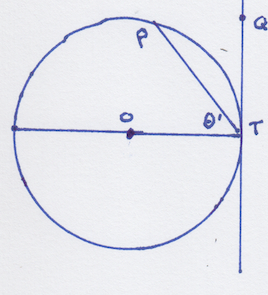
\includegraphics [scale=0.6] {U1.png} \end{center}
We want to find the angle formed with a chord of the circle like $PT$.  Let that angle be $\theta$ and then, because space is a bit tight, label its complementary angle $\theta'$.

$\theta'$ subtends the arc from $P$ counter-clockwise to where the diameter meets the circle on the left.  But $\angle OTQ$ is a right angle, $\theta + \theta' = 90$.  It's clear that $\theta$ subtends the arc $PT$, as expected.  Twice $\theta$ will be equal to the length of the arc $PT$.

\subsection*{crossed chords}
Two chords cross in a circle.  We already know a theorem about the parts of the chords, but this question is about angles.

\begin{center} 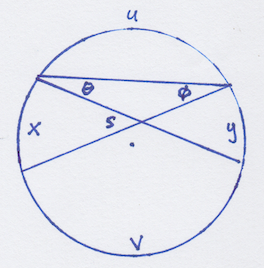
\includegraphics [scale=0.6] {U2.png} \end{center}

One of the angles where the two chords cross is $s$.  What is $\theta$ in terms of the arcs $x$ and $y$?  We might guess.  If the arcs crossed at the center then $s$ would be exactly equal to either of the two equal arcs $x$ and $y$, so $2 s = x + y$.  

And if $s$ were on the left or right periphery then one of $x$ and $y$ would be zero and $2 s$ would be equal to the other one.  Again, $2 s = x + y$.

So we guess that $s = (x + y)/2$, $s$ is the \emph{average} of $x$ and $y$.

\emph{Proof}.

Draw the chord connecting the points on the circle delimiting one of the other arcs, for example, $v$.  Then, $s$ is the exterior angle for this triangle, so it is equal to the two new angles formed by the chord.  
\begin{center} 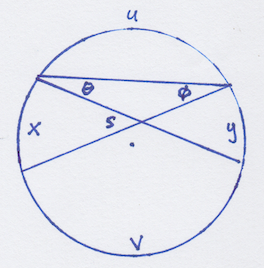
\includegraphics [scale=0.6] {U2.png} \end{center}
We have:
\[ s = \theta + \phi \]
but $2 \theta = x$ and $2 \phi = y$ so
\[ x + y = 2  \theta + 2 \phi = 2s \]

$\square$

One can also work with $x$ or $y$ and use the triangle sum theorem.  Draw the chord corresponding to arc $x$.  (Not shown).  Then
\[ u/2 + v/2 + s = 180 \]
\[ u + v + 2s = 360 \]
But the sum of the arcs is equal to that:
\[ u + v + x + y = 360 \]
Hence
\[ 2s = x + y \]

\subsection*{Chords from an external point}

Two chords are drawn extending out to the same external point, $P$.  We already know a theorem about the segments of these secant lines, but this question is about arcs and angles.
\begin{center} 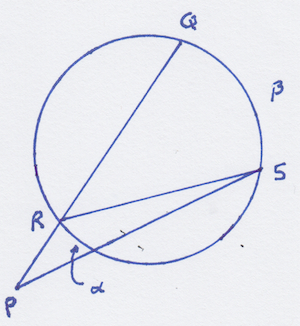
\includegraphics [scale=0.6] {U3.png} \end{center}
What can we say about the angle $P$ in terms of the arcs $\alpha$ and $\beta$?

We might guess here as well.  If $P$ were on the circle then $2P$ would just be $\beta$.  Since $P$ is smaller than it would be if on the circle, we'll need to subtract something from $\beta$.  On the other hand if $P$ were very far away from the circle then $P$ would be very small, and also $\alpha$ would be very nearly equal to $\beta$.  Let's see.

Draw $RS$.  $\angle QRS$ subtends arc $\beta$ so $2 \angle QRS = \beta$.

Since $\angle QRS$ is the exterior angle for $\triangle PRS$, we know that $\angle QRS = P + S$ so
\[ \beta = 2 \angle QRS = 2P + 2S \]
Finally, we have that $2S = \alpha$.
\[ \beta = 2P + \alpha \]
\[ P = \frac{\beta - \alpha}{2} \]
We subtract the arc that the angle subtends going in the "wrong" direction.

\end{document}
